% !TeX root = main.tex
\lecture{16}{Tue 17 Mar 2026 11:00}{Orbits II: Orbits in Attractive Potentials }

Recap from last lecture:
\begin{itemize}
    \item The magnitude of the angular momentum is conserved: $l = mr^2 \dot{\theta}$.
    \item Total energy is conserved:
    \[
        E = \frac{1}{2} m \dot{r}^2 + \frac{l^2}{2mr^2} + V(r)
    \]
    This is called the radial energy equation.
\end{itemize}

\section{Interpreting the Radial Energy Equation}
For a central conservative potential (fixed energy):
\[
    E = \frac{1}{2} m \dot{r}^2 + \frac{l^2}{2mr^2} + V(r)
\]

This equation tells us about the behaviour of a particle with constant energy and angular momentum in a radial potential.

The second term looks like a strong repulsive force at a small radius. It effectively flings the particle away if it gets too close. It has the same form as the fictional centrifugal force, so is called centrifugal potential.

We often lump the last two terms together to the ``effective potential'':
\[
    E = \frac{1}{2} m \dot{r}^2 + \underbrace{\frac{l^2}{2mr^2} + V(r)}_\text{effective potential, $V_\text{eff}$}
\]

Total energy is conserved (so does not rely on $r$) but the effective potential does. The effective potential gives the minimum possible energy that an object can have with radius of orbit $r$ and angular momentum $l$. The first term is zero in circular motion (ideal low energy case).

More generally in the non-circular case, the object occupies the space above an ideal sketch for the circular case.

\section{Consequences for Attractive Potentials}
Note that attractive potentials are negatively signed.

\subsection{Example 1: $V(r) = -k/r^3$, where $k \in \R$}
In terms of a force:
\[
\underline{F}(\underline{r}) = -\nabla V = - \frac{\partial V}{\partial r} \hat{\underline{r}} = \frac{3k}{r^4} \hat{\underline{r}}
\]

The effective potential is given by:
\[
    V_{\text{eff}} = \frac{l^2}{2mr^2} - \frac{k}{r^3}
\]

We want to understand the shape of $V_\text{eff} = \frac{l^2}{2mr^2} - \frac{k}{r^3}$ by finding its asymptotes, axis crossings, and turning points in order to sketch it.

\textbf{Asymptotes}

As $r \to \infty$, $V_\text{eff} \to \frac{l^2}{2mr^2} \to 0$ (from above).

As $r \to 0$, $V_\text{eff} \to \frac{-k}{r^3} \to - \infty$.

\textbf{Turning Points}

\[
    \frac{\partial V_\text{eff}}{\partial r} = -\frac{2l^2}{2mr^3} + \frac{3k}{r^4}
\]
This is zero when $r = \frac{3mk}{l^2}$

Assembling these gives:
\begin{figure}[H]
    \centering
    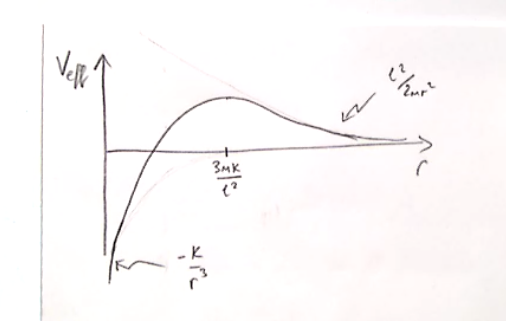
\includegraphics[width=0.75\textwidth]{figures/lec16_01.png}
     \caption{}
\end{figure}

As the particle has a combination of potential and kinetic energy, the orbiting particle must have energy lying above this curve. At lowest, when it has no kinetic energy (purely potential) it can lie on this curve, but not below.

There are multiple different particles subject to this effective potential depending on its energy. The maximum value of the potential curve is denoted $E_\text{max}$, and the particle has energy $E$.

\begin{itemize}
    \item If $E > E_\text{max}$.
    \item If $E < 0$, the particle is always captured and sucked in.
    \item If $0 < E < E_\text{max}$, the particle is either sucked in (down the LHS) or expelled to infinity (along the RHS).
\end{itemize}

This means that we're dealing with a case where there is no stable possible orbit. This is true for all $V(r) \propto r^{-n}$ where $n \in \R_{\geq 3}$.

\subsection{Example 2: $V(r) = -k/r^2$, where $k \in \R$}
Depending on the sign of the constants, this gives an effectively $1/r^2$ potential curve. The potential is always positive or always negative, which again results in no stable possible orbits.

\subsection{Example 3: $V(r) = -k/r$, where $k \in \R$}

\[
    V(r) = \frac{-k}{r}
\]
\[
    \implies F(r) = \frac{\partial V}{\partial r} = \frac{k}{r^2}
\]

Hence:
\[
    V_\text{eff}(r) = \frac{l}{2mr^2} - \frac{k}{r}
\]

This time, as:
\begin{itemize}
    \item $r \to \infty$: $V_\text{eff} \to - \frac{k}{r} \to 0$ from below.
    \item $r \to 0$: $V_\text{eff} \to \frac{l^2}{2 m r^2} \to + \infty$.
\end{itemize}

And turning points:
\[
    \frac{\partial V_\text{eff}}{\partial r} = - \frac{2 l^2}{2 m r^3} + \frac{k}{r^2}
\]
\[
    = 0 \text{ when } r_\text{min} = \frac{l^2}{mk}
\]

As the curve tends to zero from below at infinity, and to infinity at zero, the turning point must be a minimum. This minimum value at $r = r_\text{min}$.

\[
    V_\text{eff}(r_\text{min}) = \frac{l^2}{2m} \left(\frac{m^2k^2}{l^4}\right) - \frac{mk^2}{l^2}
\]
\[
    V_\text{eff}(r_\text{min} = \frac{mk^2}{2l^2} - \frac{mk^2}{l^2})
\]

And finally the x-axis crossing:
\[
    V_\text{eff}(r) = 0 - \frac{l^2}{2mr^2} - \frac{k}{r}
\]
\[
    \text{when: } r = \frac{l^2}{2mk^2}
\]

And finally putting this all together:
\begin{figure}[H]
    \centering
    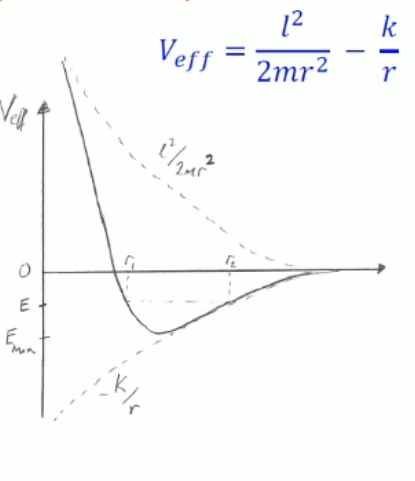
\includegraphics[width=0.75\textwidth]{figures/lec16_02.png}
     \caption{}
\end{figure}

This creates a small stable potential well where the orbiting object is bound. Depending on the particle energy, we have a few different cases:
\begin{itemize}
    \item $E < E_\text{min}$: This is not possible. The particle must always have total energy exceeding the minimum potential energy.
    \item $E = E_\text{min} = - \frac{-mk^2}{2l^2}$: The particle is in a perfect circular orbit. This is the lowest possible potential state, which (as demonstrated before) requires a fixed $\vec{r}$ circular path.
    \item $E_\text{min} < E < 0$: This is an orbit where the particle is trapped in a stable orbit. The orbit is elliptical, as the particle travels up/down the potential it transfers between kinetic and potential.
    
    \begin{enumerate}
        \item In the diagram, with the value of E chosen, the potential is maximum for this $E$ at $r_1, r_2$. Here the energy is only potential. For all other values, $E > V_\text{eff}$.
        \item This gives an elliptical orbit with $r_1$ and $r_2$ as the semiminor and semimajor axes.
    \end{enumerate}
    \item When $E = 0$ the particle just barely escapes. It takes a parabolic path.
    \item When $E > 0$, the particle is certain to escape. It takes a hyperbolic path.

\end{itemize}

Note that as angular momentum increases, the minimum moves to a larger and larger radius and becomes less and less negative.

\section{Parametrising an Ellipse}
\subsection{Hyperbolic Orbits}
When $E > 0$, we have a hyperbolic orbit. This is an unbound object that comes in from infinity, swings around the central object and back out to infinity without being captured.

\subsection{Parabolic Orbits}
When $E = 0$, we have a parabolic orbit. This is the boundary case where the object just barely escapes. It comes in from infinity, swings around the central object and back out to infinity, but it takes an infinitely long time to do so.

\subsection{Bound Elliptical Orbits}
When $E<0$ we have an elliptical orbit (or a circular orbit which is a special case of an ellipse). This is a bound object that is captured by the central object and orbits around it indefinitely.

We can parametrise the ellipse by:
\begin{itemize}
    \item The shortest distancce from the ellipse to the centre, the semi-minor axis $b$.
    \item The longest distance from the ellipse to the centre, the semi-major axis $a$.
    \item The eccentricity $e$, which is a measure of how much the ellipse deviates from a circle. It is defined as $e = \frac{a - b}{a + b}$. For a circle, $a = b$ so $e = 0$. 
\end{itemize}

For an ellipse centred on the origin, the equation for an ellipse is given by:
\[
    \frac{x^2}{a^2} + \frac{y^2}{b^2} = 1
\]

Considering one focus on the ellipse at the origin, we now have:
\[
    \frac{(x - a \epsilon)^2}{a^2} + \frac{y^2}{b^2} = 1
\]

The distance from the focus to the centre is $\epsilon a$.

The closest point on the ellipse to the focus is the perigee, at $r = (1 - \epsilon)a$ and the furthest point is the apogee, at $r = (1 + \epsilon)a$.
